\chapter{Physique nucléaire}\label{ch:b3:nuclear-physics}

% Provenance (not for print): first half of the "physique subatomique"
% module common to the surveyed third-year curricula; particle physics
% follows in the next chapter. Deepens the high-school volume's
% radioactivity with SEMF, Gamow tunnelling and reactor physics.

Le volume de lycée en a raconté les grandes lignes~: les atomes ont
un noyau~; certains noyaux se délitent, sur des horaires allant de la
microseconde au milliard d'années~; et des grammes de matière cachent
des mégatonnes d'énergie. Ce chapitre rouvre le noyau avec les outils
de troisième année. Un modèle de goutte à cinq termes prédit au pour
cent près la liaison de centaines de \omterm{def:b3:nuclear-physics:nuclide}{nucléides}~; l'effet tunnel ---
le problème de la barrière du volume de deuxième année, promu ---
explique comment une seule formule couvre vingt-cinq ordres de
grandeur de durées de vie en désintégration $\alpha$~; et le maximum
discret de la courbe d'\omterm{prop:b3:nuclear-physics:binding}{énergie de liaison}, au fer, partage toute la
technologie nucléaire en deux camps~: casser le lourd (les
réacteurs) ou joindre le léger (les étoiles, et un jour des
centrales). Le chapitre s'achève au bord d'une piscine de réacteur,
qui luit d'un bleu Tcherenkov.

\section{Le noyau~: une goutte saturée}

\begin{definition}[Nucléides, taille et densité]\label{def:b3:nuclear-physics:nuclide}
\index{nucléide}\index{isotope}\index{rayon nucléaire}
Un \emph{nucléide} $^{A}_{Z}\text{X}$ contient $Z$ protons et $N = A -
Z$ neutrons, liés par l'\emph{interaction forte}~: intense
(${\sim}\qty{100}{}\times$ Coulomb au contact), de courte portée
(${\sim}\qty{1}{fm}$, ressentie des seuls voisins qui se touchent)
et aveugle à la charge (elle agrippe protons et neutrons pareillement).
Les expériences de diffusion donnent à tout noyau la même recette~:
un rayon
\[
R = r_0A^{1/3} , \qquad r_0 \approx \qty{1.2}{fm} ,
\]
si bien que le volume croît comme $A$ et que la densité est un
universel $\rho \approx \qty{2.3e17}{kg/m^3}$ --- une goutte de pluie
de cette matière pèserait comme une flotte de pétroliers, et le
\cref{ch:b3:astrophysics} rencontrera des étoiles entières à cette
densité. Les \emph{isotopes} partagent $Z$ mais diffèrent par $N$~:
même chimie, destins nucléaires différents.
\end{definition}

\begin{proposition}[Défaut de masse et énergie de liaison]\label{prop:b3:nuclear-physics:binding}
\index{défaut de masse}\index{énergie de liaison}\index{pic du fer}
Un noyau lié pèse \emph{moins} que ses constituants~; d'après le
\cref{ch:b3:relativistic-dynamics}, la masse manquante est l'\omterm{prop:b3:nuclear-physics:binding}{énergie
de liaison},
\[
B = \big(Zm_{\text{p}} + Nm_{\text{n}} - m_{\text{noyau}}\big)c^2 ,
\]
typiquement ${\sim}\qty{8}{MeV}$ \emph{par nucléon} --- un million de
fois la chimie. Tracé par nucléon, $B/A$ monte fortement à travers les noyaux légers
(les effets de surface s'estompent), culmine à
$\approx\qty{8.8}{MeV}$ près du fer 56, puis dérive vers le bas à
mesure que la répulsion coulombienne, de longue portée et sans
saturation, taxe les poids lourds. Les deux pentes sont des mines
d'énergie~: la \emph{fusion} gravit la pente de gauche (l'affaire du
Soleil), la \emph{fission} descend celle de droite (celle du
réacteur) --- et le fer, au sommet, est la cendre nucléaire des deux.
\end{proposition}

\begin{omfigure}
\begin{tikzpicture}
  \begin{axis}[omaxis, axis x line=bottom, axis y line=left,
    width=11.2cm, height=6.2cm, xmin=0, xmax=250, ymin=0, ymax=10.3,
    xlabel={nombre de masse $A$}, ylabel={$B/A$ (\unit{MeV})},
    xlabel style={at={(axis description cs:0.5,-0.1)}, anchor=north},
    xtick={56,100,150,200,238}, ytick={2,4,6,8}, clip=false]
    \addplot[omDef, very thick, smooth] coordinates {
      (2,1.11) (3,2.7) (6,5.3) (9,6.46) (12,7.68) (16,7.98)
      (24,8.26) (40,8.55) (56,8.79) (75,8.7) (100,8.6)
      (125,8.45) (150,8.3) (175,8.1) (200,7.9) (220,7.75) (238,7.57)};
    \fill[omThm] (axis cs:4,7.07) circle (1.6pt);
    \draw[gray, thin] (axis cs:12.5,6.85) -- (axis cs:5.2,7.02);
    \node[omThm, font=\scriptsize, anchor=west] at (axis cs:13,6.8)
      {$^4$He};
    \fill[omThm] (axis cs:56,8.79) circle (1.6pt);
    \node[omThm, font=\scriptsize, anchor=south] at (axis cs:56,9.0)
      {$^{56}$Fe~: le sommet};
    \fill[omThm] (axis cs:238,7.57) circle (1.6pt);
    \node[omThm, font=\scriptsize, anchor=south west] at (axis cs:225,7.85)
      {$^{238}$U};
    \draw[->, omExo, thick] (axis cs:14,4.0) -- (axis cs:40,6.4);
    \node[omExo, font=\scriptsize, anchor=west] at (axis cs:18,3.6)
      {la fusion gravit};
    \draw[->, omExo, thick] (axis cs:225,6.4) -- (axis cs:130,7.6);
    \node[omExo, font=\scriptsize, anchor=east] at (axis cs:242,5.9)
      {la fission descend};
  \end{axis}
\end{tikzpicture}

{\small La courbe d'\omterm{prop:b3:nuclear-physics:binding}{énergie de liaison} --- sans doute le graphique le
plus lourd de conséquences de la physique. Les noyaux légers gagnent
à fusionner, les lourds à se scinder~; par kilogramme, la pente de
gauche paie environ quatre fois mieux, et le Soleil s'y tient.}
\end{omfigure}

\begin{proposition}[La formule de masse semi-empirique]\label{prop:b3:nuclear-physics:semf}
\index{formule de masse semi-empirique}\index{vallée de stabilité}
Modélisez le noyau comme une goutte de liquide chargée et toute la
courbe découle de cinq termes~:
\[
B = a_{\text{V}}A - a_{\text{S}}A^{2/3}
- a_{\text{C}}\frac{Z^2}{A^{1/3}}
- a_{\text{A}}\frac{(A - 2Z)^2}{A} + \delta(A) ,
\]
avec (en \unit{MeV}) $a_{\text{V}} = 15.8$ (chaque nucléon se lie à
ses voisins~: le volume), $a_{\text{S}} = 17.8$ (les nucléons de
surface se lient moins~: la «~tension superficielle~» de la goutte),
$a_{\text{C}} = 0.71$ (Coulomb, le saboteur à longue portée),
$a_{\text{A}} = 23.7$ (asymétrie~: d'après le
\cref{ch:b3:quantum-statistics}, protons et neutrons remplissent deux
échelles de Fermi séparées, au meilleur prix quand elles sont
également pleines), et $\delta$ une petite prime d'appariement pour
les nombres pairs (\cref{ch:b3:identical-particles}). La
minimisation à $A$ fixé trace la \emph{\omterm{prop:b3:nuclear-physics:semf}{vallée de stabilité}}~:
$N \approx Z$ pour les noyaux légers, s'infléchissant vers les riches
en neutrons ($N/Z \to 1.5$) à mesure que Coulomb punit les protons
--- et les \omterm{def:b3:nuclear-physics:nuclide}{nucléides} hors vallée y retombent par désintégration
$\beta$.
\end{proposition}
\admitted

\begin{omfigure}
\begin{tikzpicture}
  \begin{axis}[omaxis, axis x line=bottom, axis y line=left,
    width=8.6cm, height=6.4cm, xmin=0, xmax=95, ymin=0, ymax=150,
    xlabel={protons $Z$}, ylabel={neutrons $N$},
    xlabel style={at={(axis description cs:0.5,-0.1)}, anchor=north},
    xtick={20,40,60,80}, ytick={50,100,150}, clip=true]
    \addplot[gray, dashed, domain=0:95] {x};
    \addplot[omDef, very thick, domain=1:92, samples=100]
      {x + 0.03*x^(5/3)};
    \node[gray, font=\scriptsize, anchor=north west] at
      (axis cs:78,74) {$N = Z$};
    \node[omDef, font=\scriptsize, anchor=north west, align=left] at
      (axis cs:48,125) {vallée de\\stabilité};
    \fill (axis cs:26,30) circle (1.5pt);
    \node[font=\scriptsize, anchor=north west] at (axis cs:26,29) {Fe};
    \fill (axis cs:92,146) circle (1.5pt);
    \node[font=\scriptsize, anchor=north west] at (axis cs:88,143) {U};
  \end{axis}
\end{tikzpicture}

{\small La \omterm{prop:b3:nuclear-physics:semf}{vallée de stabilité}. Les noyaux légers équilibrent leurs
deux échelles de Fermi ($N = Z$)~; les lourds diluent leur facture
coulombienne avec des neutrons supplémentaires. Un \omterm{def:b3:nuclear-physics:nuclide}{nucléide} hors du
fond de la vallée y revient par désintégration $\beta$ --- et les
fragments de fission, nés bien au-dessus de la ligne, sont
furieusement radioactifs pour exactement cette raison.}
\end{omfigure}

\section{La radioactivité, montre en main}

\begin{theorem}[La loi de décroissance]\label{thm:b3:nuclear-physics:decay}
\index{loi de décroissance radioactive}\index{demi-vie}\index{activité}
Un noyau instable n'a ni mémoire ni vieillissement~: à chaque seconde
qu'il vit, il se désintègre avec la même probabilité $\lambda$. Pour
$N$ noyaux, $\dd N = -\lambda N\,\dd t$, donc
\[
N(t) = N_0\,\eu^{-\lambda t} = N_0\,2^{-t/T_{1/2}} ,
\qquad T_{1/2} = \frac{\ln2}{\lambda} ,
\]
et l'\emph{activité} $\mathcal A = \lambda N$ (désintégrations par
seconde, \unit{Bq}) s'éteint sur la même exponentielle. Les demi-vies
vont de la microseconde au milliard d'années~; la statistique du
\cref{ch:b3:microcanonical-ensemble} garantit que, si un noyau isolé
est parfaitement imprévisible, une mole d'entre eux tient le temps
exponentiel mieux qu'aucune horloge --- le fondement de la datation
radiométrique.
\end{theorem}

\begin{proof}
Une probabilité constante par seconde signifie $N(t + \dd t) = N(t)(1 -
\lambda\dd t)$~; intégrer. Poser $N/N_0 = \tfrac12$ donne
$T_{1/2}$.
\end{proof}

\begin{omfigure}
\begin{tikzpicture}
  \begin{axis}[omaxis, axis x line=bottom, axis y line=left,
    width=9.8cm, height=5.6cm, xmin=0, xmax=4.3, ymin=0, ymax=1.12,
    xlabel={$t/T_{1/2}$}, ylabel={$N/N_0$},
    xlabel style={at={(axis description cs:0.5,-0.1)}, anchor=north},
    xtick={1,2,3,4}, ytick={0.25,0.5,1},
    yticklabels={$\tfrac14$,$\tfrac12$,$1$}, clip=true]
    \addplot[omDef, very thick, domain=0:4.3, samples=150]
      {exp(-0.6931*x)};
    \draw[gray, dashed] (axis cs:0,0.5) -| (axis cs:1,0);
    \draw[gray, dashed] (axis cs:0,0.25) -| (axis cs:2,0);
    \node[font=\scriptsize, anchor=south west, align=left] at
      (axis cs:2.3,0.55) {chaque demi-vie\\divise le compte par deux};
  \end{axis}
\end{tikzpicture}

{\small Décroissance exponentielle~: des individus sans mémoire, une
population ponctuelle. Deux demi-vies laissent un quart~; dix en
laissent un millième --- la règle avec laquelle les physiciens datent
le charbon de bois, les glaciers et la Terre.}
\end{omfigure}

\begin{remark}[Trois portes de sortie d'un noyau]\label{rem:b3:nuclear-physics:modes}
\index{désintégration alpha}\index{désintégration bêta}\index{désintégration gamma}\index{modèle de Gamow}
$\boldsymbol\alpha$~: un noyau lourd émet un agrégat $^4$He.
Classiquement impossible --- la barrière coulombienne culmine à
\qty{25}{MeV} et l'$\alpha$ part avec \qty{5}{}--\qty{9}{MeV} ---
cela se produit par \emph{effet tunnel} (la barrière du volume de
deuxième année, incurvée)~: la sensibilité exponentielle de Gamow
change un facteur deux en énergie en vingt ordres de grandeur de
durée de vie, exactement le schéma de Geiger--Nuttall
(\cref{exo:b3:nuclear-physics:8}).
$\boldsymbol\beta$~: un neutron devient un proton (ou l'inverse), en
émettant un électron (ou un positon) et un neutrino ---
l'\emph{interaction faible} à l'œuvre, la force qui ramène dans la
vallée~; l'histoire du neutrino attend le
\cref{ch:b3:particle-physics}.
$\boldsymbol\gamma$~: un noyau excité largue des photons de
\unit{MeV}, l'analogue nucléaire des raies spectrales du
\cref{ch:b3:hydrogen-atom}. Les désintégrations s'enchaînent
jusqu'au fond de la vallée~: l'échelle de l'uranium s'achève, quatorze
barreaux plus loin, sur du plomb stable.
\end{remark}

\section{Descendre les pentes~: fission et fusion}

\begin{proposition}[Fission et réaction en chaîne]\label{prop:b3:nuclear-physics:fission}
\index{fission}\index{réaction en chaîne}\index{masse critique}
Un neutron lent absorbé par l'$^{235}$U fait une goutte oscillante
qui se scinde~: deux fragments de masse moyenne, deux à trois
neutrons frais, et $\approx\qty{200}{MeV}$ --- l'écart de $B/A$ entre
les \qty{7.6}{MeV} de l'uranium et les \qty{8.5}{MeV} des fragments,
multiplié par 235. Les neutrons libérés peuvent fissionner d'autres
noyaux~: avec un facteur de multiplication $k$ (neutrons par neutron,
une génération plus tard), une population croît comme $k^n$ ---
sous-critique ($k < 1$) elle s'éteint, critique ($k = 1$) elle tient,
surcritique elle explose. Un réacteur modère les neutrons jusqu'aux
vitesses lentes (le régime préféré de la fission), s'appuie sur les
0,7\,\% de neutrons qui arrivent avec \emph{des secondes} de retard,
issus des désintégrations de fragments --- le délai qui rend
$k \approx 1$ humainement réglable --- et laisse les barres de
contrôle manger le surplus (\cref{pb:b3:nuclear-physics:1}).
\end{proposition}
\admitted

\begin{omfigure}
\begin{tikzpicture}[scale=1.0]
  % stage 1: nucleus + neutron
  \draw[->, thick] (-1.3,0) -- (-0.55,0);
  \fill[gray] (-1.55,0) circle (2.6pt);
  \node[font=\scriptsize, anchor=south] at (-1.55,0.12) {n};
  \draw[omDef, fill=omDef!15, thick] (0.35,0) circle (0.62);
  \node[omDef, font=\scriptsize] at (0.35,0) {$^{235}$U};
  % arrow
  \draw[->, thick] (1.35,0) -- (2.05,0);
  % stage 2: deformed drop (peanut)
  \draw[omDef, fill=omDef!15, thick, rotate around={0:(3.1,0)}]
    (3.1,0) ellipse (0.85 and 0.42);
  \draw[omDef!60, dashed] (3.1,-0.5) -- (3.1,0.5);
  % arrow
  \draw[->, thick] (4.3,0) -- (5.0,0);
  % stage 3: fragments + neutrons
  \draw[omThm, fill=omThm!12, thick] (5.9,0.55) circle (0.42);
  \draw[omThm, fill=omThm!12, thick] (5.9,-0.55) circle (0.42);
  \node[omThm, font=\tiny] at (5.9,0.55) {Ba};
  \node[omThm, font=\tiny] at (5.9,-0.55) {Kr};
  \foreach \ang in {15,-8,40}{
    \fill[gray] ({6.7+0.35*cos(\ang)},{0.3*sin(\ang)}) circle (2.2pt);
    \draw[->, gray] ({6.95+0.35*cos(\ang)},{0.32*sin(\ang)}) --
      ({7.55+0.35*cos(\ang)},{0.42*sin(\ang)});}
  \node[font=\scriptsize, anchor=west, align=left] at (8.05,0)
    {2--3 neutrons\\$+\ \qty{200}{MeV}$};
\end{tikzpicture}

{\small Fission en goutte liquide~: un neutron lent met l'$^{235}$U
en oscillation~; la répulsion coulombienne de la goutte déformée
l'emporte sur sa tension superficielle, et elle se déchire en
fragments riches en neutrons plus les neutrons de reste qui rendent
une chaîne possible.}
\end{omfigure}

\begin{remark}[La fusion~: la pente plus rude et meilleure]\label{rem:b3:nuclear-physics:fusion}
\index{fusion}
Joindre des noyaux légers paie $\sim4\times$ plus par kilogramme que
scinder des lourds, et sans fragments à longue vie --- mais les
réactifs, tous deux positifs, doivent franchir par effet tunnel leur
barrière coulombienne mutuelle, ce qui exige des températures de
$10^7$--$10^8\,\unit{K}$ (\cref{exo:b3:nuclear-physics:11}). Les
étoiles y parviennent en étant énormes (\cref{ch:b3:astrophysics}~:
le Soleil change \qty{600}{} millions de tonnes d'hydrogène en hélium
chaque seconde)~; les laboratoires s'y essaient avec des plasmas mis
en bouteille magnétique et, jusqu'ici, un bilan énergétique encore en
deçà de ses ambitions de seuil de rentabilité.
\end{remark}

\begin{omfigure}
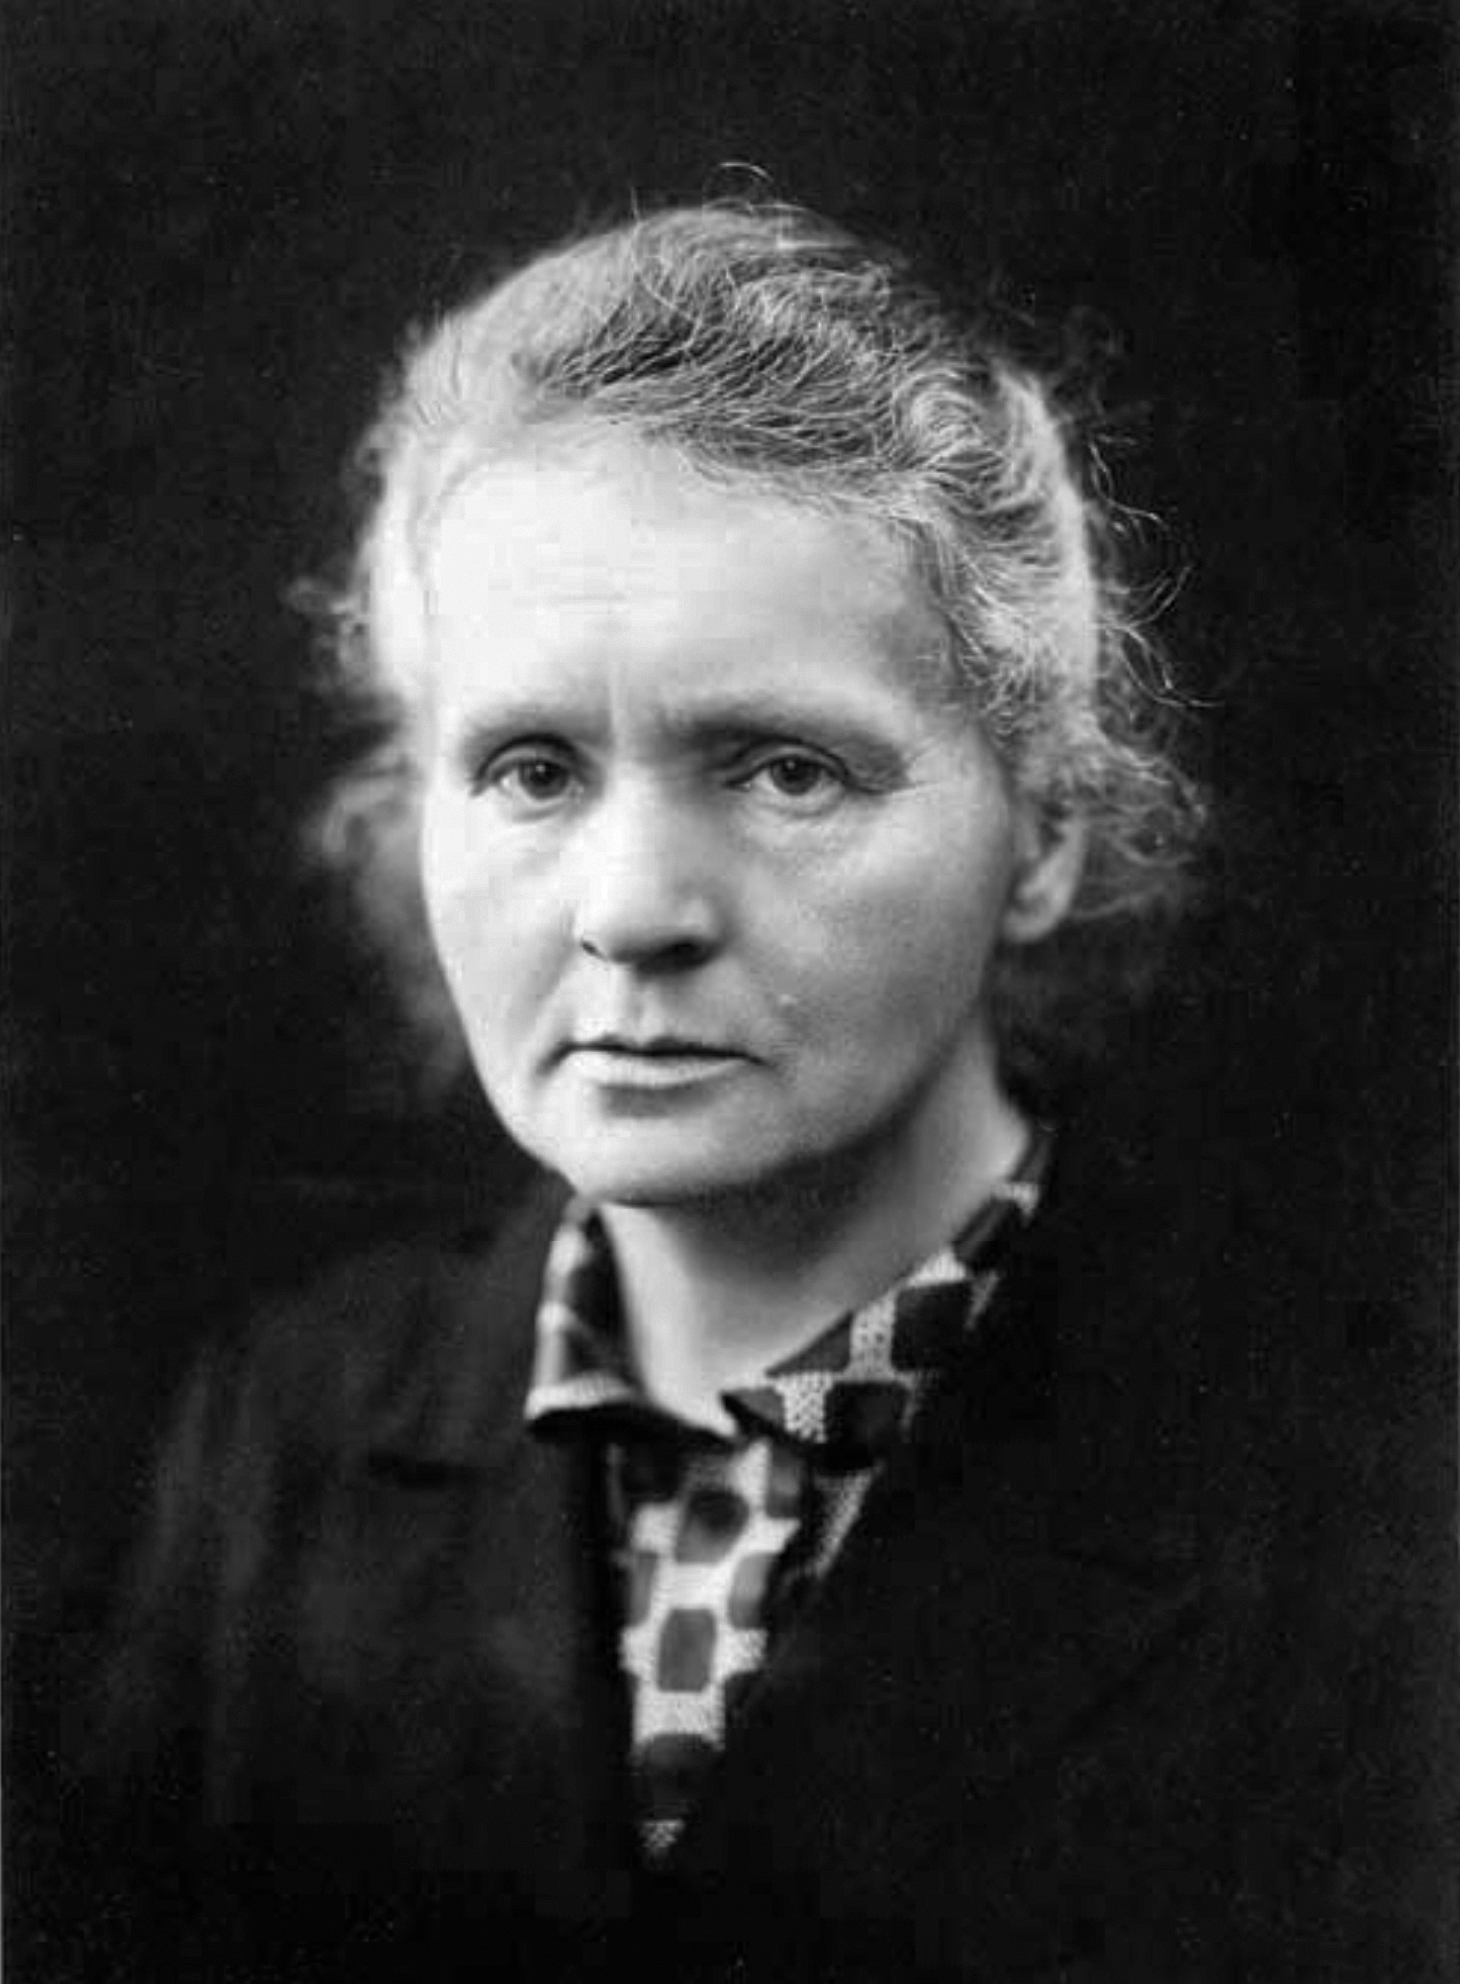
\includegraphics[width=0.34\linewidth]{images/book5/photo-marie-curie.jpg}

{\small Marie Curie (photographie d'Henri Manuel, vers 1920, domaine public)~: deux fois lauréate du prix Nobel pour avoir ouvert le sujet de ce chapitre --- le gramme de radium de \cref{exo:b3:nuclear-physics:4} était le sien.}
\end{omfigure}

\section{Exercices}

\begin{exercise}[$\star$]\label{exo:b3:nuclear-physics:1}
Comptabilité. (a) Donner $Z$, $N$, $A$ pour $^{12}$C, $^{14}$C,
$^{235}$U, $^{238}$U. (b) Quelles paires sont des \omterm{def:b3:nuclear-physics:nuclide}{isotopes}~? (c)
Pourquoi les \omterm{def:b3:nuclear-physics:nuclide}{isotopes} partagent-ils la chimie mais non la stabilité
nucléaire~? (d) $^{14}$C et $^{14}$N partagent $A = 14$~: comment
appelle-t-on de tels \omterm{def:b3:nuclear-physics:nuclide}{nucléides}, et quelle désintégration les relie~?
\end{exercise}

\begin{exercise}[$\star$]\label{exo:b3:nuclear-physics:2}
La densité universelle. (a) À partir de $R = r_0A^{1/3}$, montrer que
la densité nucléaire est indépendante de $A$ et l'évaluer. (b)
Calculer la masse d'une cuillerée (\qty{5}{mL}) de matière nucléaire.
(c) Quelle fraction du volume d'un atome son noyau occupe-t-il
(prendre $R_{\text{atome}} = \qty{1e-10}{m}$, $A = 60$)~? (d) Que dit
la loi en $A^{1/3}$ elle-même sur la portée de la force forte~?
\end{exercise}

\begin{exercise}[$\star$]\label{exo:b3:nuclear-physics:3}
Peser la colle. Masses nucléaires~: $m_{\text{p}} =
\qty{1.007276}{u}$, $m_{\text{n}} = \qty{1.008665}{u}$,
$m(^4\text{He}) = \qty{4.001506}{u}$~;
$\qty{1}{u}\,c^2 = \qty{931.5}{MeV}$. (a) Calculer le \omterm{thm:b3:relativistic-dynamics:emc2}{défaut de masse}
et l'\omterm{prop:b3:nuclear-physics:binding}{énergie de liaison} de l'$^4$He. (b) Donner $B/A$. (c) Comparer
$B$ aux \qty{13.6}{eV} du \cref{ch:b3:hydrogen-atom}~: combien
d'ordres de grandeur séparent la colle nucléaire de la colle
atomique~? (d) Pourquoi la liaison exceptionnelle de l'$^4$He (le pic
de la figure) en fait-elle la monnaie de la désintégration $\alpha$~?
\end{exercise}

\begin{exercise}[$\star$]\label{exo:b3:nuclear-physics:4}
Le premier curie. Le radium 226~: $T_{1/2} = 1600$ ans, masse molaire
\qty{226}{g/mol}. Pour un gramme~: (a) compter les noyaux~; (b)
calculer $\lambda$~; (c) calculer l'activité et comparer à l'unité
historique $1\,\text{Ci} = \qty{3.7e10}{Bq}$ (définie comme
exactement ce gramme)~; (d) quelle part du gramme survit après
4800 ans~?
\end{exercise}

\begin{exercise}[$\star\star$]\label{exo:b3:nuclear-physics:5}
La formule à l'œuvre. Avec $a_{\text{V}} = 15.75$,
$a_{\text{S}} = 17.8$, $a_{\text{C}} = 0.711$,
$a_{\text{A}} = 23.7$ (\unit{MeV}) et un appariement de
$+12/\sqrt A$ pour les noyaux pairs--pairs~: (a) calculer les quatre
termes principaux de $B$ pour le $^{56}$Fe ($Z = 26$). (b) Sommer
(appariement compris) et comparer $B/A$ aux \qty{8.79}{MeV}
mesurées. (c) Quels deux termes se battent le plus dur, et que fixe
leur équilibre~? (d) Pourquoi le terme coulombien, seul, doit-il
croître \emph{plus vite} que $A$~?
\end{exercise}

\begin{exercise}[$\star\star$]\label{exo:b3:nuclear-physics:6}
Le fond de la vallée. (a) En ne gardant que les termes dépendant de
$Z$, minimiser la masse à $A$ fixé et obtenir
$Z^* = \dfrac{A/2}{1 + a_{\text{C}}A^{2/3}/4a_{\text{A}}}$. (b)
Évaluer pour $A = 101$ et comparer au ruthénium ($Z = 44$).
(c) Montrer que la limite des petits $A$ est $Z^* = A/2$ et
interpréter avec les deux échelles de Fermi. (d) Un fragment de
fission a $A = 95$, $Z = 36$~: à quelle distance de la vallée est-il,
et quelle suite de désintégrations s'ensuit~?
\end{exercise}

\begin{exercise}[$\star\star$]\label{exo:b3:nuclear-physics:7}
Le radiocarbone. La matière vivante maintient son $^{14}$C
($T_{1/2} = 5730$ ans) à 1 atome pour $10^{12}$ carbones~; la mort
arrête le réapprovisionnement. (a) Un échantillon de charbon de bois
montre 30\,\% de l'activité vivante~: quel âge a le feu~? (b) Un
gramme de carbone vivant~: calculer son activité en $^{14}$C
($\approx\qty{0.23}{Bq}$ attendus). (c) Pourquoi la méthode est-elle
inutile au-delà de $\sim\qty{50000}{}$ ans~? (d) Et pourquoi
est-elle inutile pour dater les roches (quelles horloges prennent le
relais)~?
\end{exercise}

\begin{exercise}[$\star\star$]\label{exo:b3:nuclear-physics:8}
La falaise de Gamow. Le polonium 212 émet un $\alpha$ de
\qty{8.78}{MeV}~; sa barrière culmine à $\approx\qty{26}{MeV}$. (a)
Montrer que l'échappée classique est impossible, et l'entrée
classique aussi --- et pourtant il se désintègre en
\qty{0.3}{\micro s}. (b) L'$\alpha$ de l'uranium 238 emporte
\qty{4.2}{MeV} et sa demi-vie est de $4.5\times10^9$ ans~: calculer
le rapport des deux constantes de désintégration. (c) Expliquer, avec
l'exponentielle de l'effet tunnel, comment un facteur deux en énergie
achète $\sim10^{24}$ en vitesse. (d) Pourquoi la même physique
impose-t-elle sa température au cœur du Soleil~?
\end{exercise}

\begin{exercise}[$\star\star$]\label{exo:b3:nuclear-physics:9}
Deux cents millions d'électronvolts. (a) Justifier les
$\qty{200}{MeV}$ par fission à partir de la courbe $B/A$. (b)
Calculer l'énergie contenue dans un kilogramme d'$^{235}$U
entièrement fissionné, en joules et en tonnes d'équivalent pétrole
(\qty{42}{GJ/t}). (c) Une centrale de \qty{1}{GW_e} à 33\,\% de
rendement~: combien de kilogrammes d'$^{235}$U par an~? (d) Pourquoi
sont-ce les fragments, et non les neutrons, qui portent l'essentiel
des \qty{200}{MeV}, et sous quelle forme cela passe-t-il aussitôt~?
\end{exercise}

\begin{exercise}[$\star\star\star$]\label{exo:b3:nuclear-physics:10}
Apprivoiser $k$. Dans un réacteur, les neutrons prompts se
reproduisent en $\ell
\approx \qty{e-4}{s}$. (a) Avec $k = 1.001$ sur les seuls neutrons
prompts, calculer la multiplication de puissance en une seconde ---
et le verdict sur un contrôle mécanique. (b) Une fraction $\beta =
0.7\,\%$ des neutrons est \emph{retardée} de $\sim\qty{10}{s}$~:
expliquer pourquoi, pour $k - 1 < \beta$, l'horloge effective de la
chaîne devient la seconde. (c) Calculer la même multiplication sur
une seconde avec le temps de génération effectif
$\sim\qty{0.1}{s}$. (d) Dites en une phrase ce que les opérateurs de
Tchernobyl ont perdu quand leur réacteur est devenu
prompt-surcritique.
\end{exercise}

\begin{exercise}[$\star\star\star$]\label{exo:b3:nuclear-physics:11}
L'arithmétique du Soleil. Globalement,
$4\,^1\text{H} \to {}^4\text{He}$ convertit \qty{0.71}{\percent} de
la masse en énergie (\qty{26.7}{MeV}, neutrinos compris). (a) À
partir de $L_\odot =
\qty{3.8e26}{W}$, calculer la masse convertie par seconde et
l'hydrogène consommé par seconde. (b) Avec $\qty{2e30}{kg}$ de
Soleil, dont un dixième d'hydrogène de cœur brûlable (prendre une
fraction d'hydrogène $\approx0.75$)~: estimer la durée de vie. (c)
Deux protons à \qty{1.5e7}{K}~: comparer $k_{\text{B}}T$ à leur
barrière coulombienne à \qty{1}{fm} et conclure qui fait la traversée
(\cref{exo:b3:nuclear-physics:8}). (d) Pourquoi la fusion, à la
différence de la fission, ne laisse-t-elle pratiquement aucune cendre
radioactive~?
\end{exercise}

\begin{exercise}[$\star\star\star$]\label{exo:b3:nuclear-physics:12}
Médecine nucléaire. (a) Le technétium 99m ($T_{1/2} = \qty{6}{h}$,
$\gamma$ de \qty{140}{keV}) est le cheval de trait de la médecine~:
calculer le nombre de noyaux, et leur masse, derrière une injection
de \qty{500}{MBq}. (b) Expliquer pourquoi une demi-vie de six
\emph{heures} et un $\gamma$ pur sont exactement ce que veut un
diagnostic. (c) La TEP~: un positon issu du $^{18}$F s'annihile avec
un électron --- utiliser le \cref{ch:b3:relativistic-dynamics} pour
donner l'énergie et la géométrie des deux photons, et donc le principe
du détecteur. (d) La radiothérapie délivre \qty{2}{Gy} (\unit{J/kg})
à une tumeur~: comparer l'énergie à une gorgée d'eau tiède, et
réconcilier l'innocuité des joules avec la létalité de l'ionisation.
\end{exercise}

\begin{omfigure}
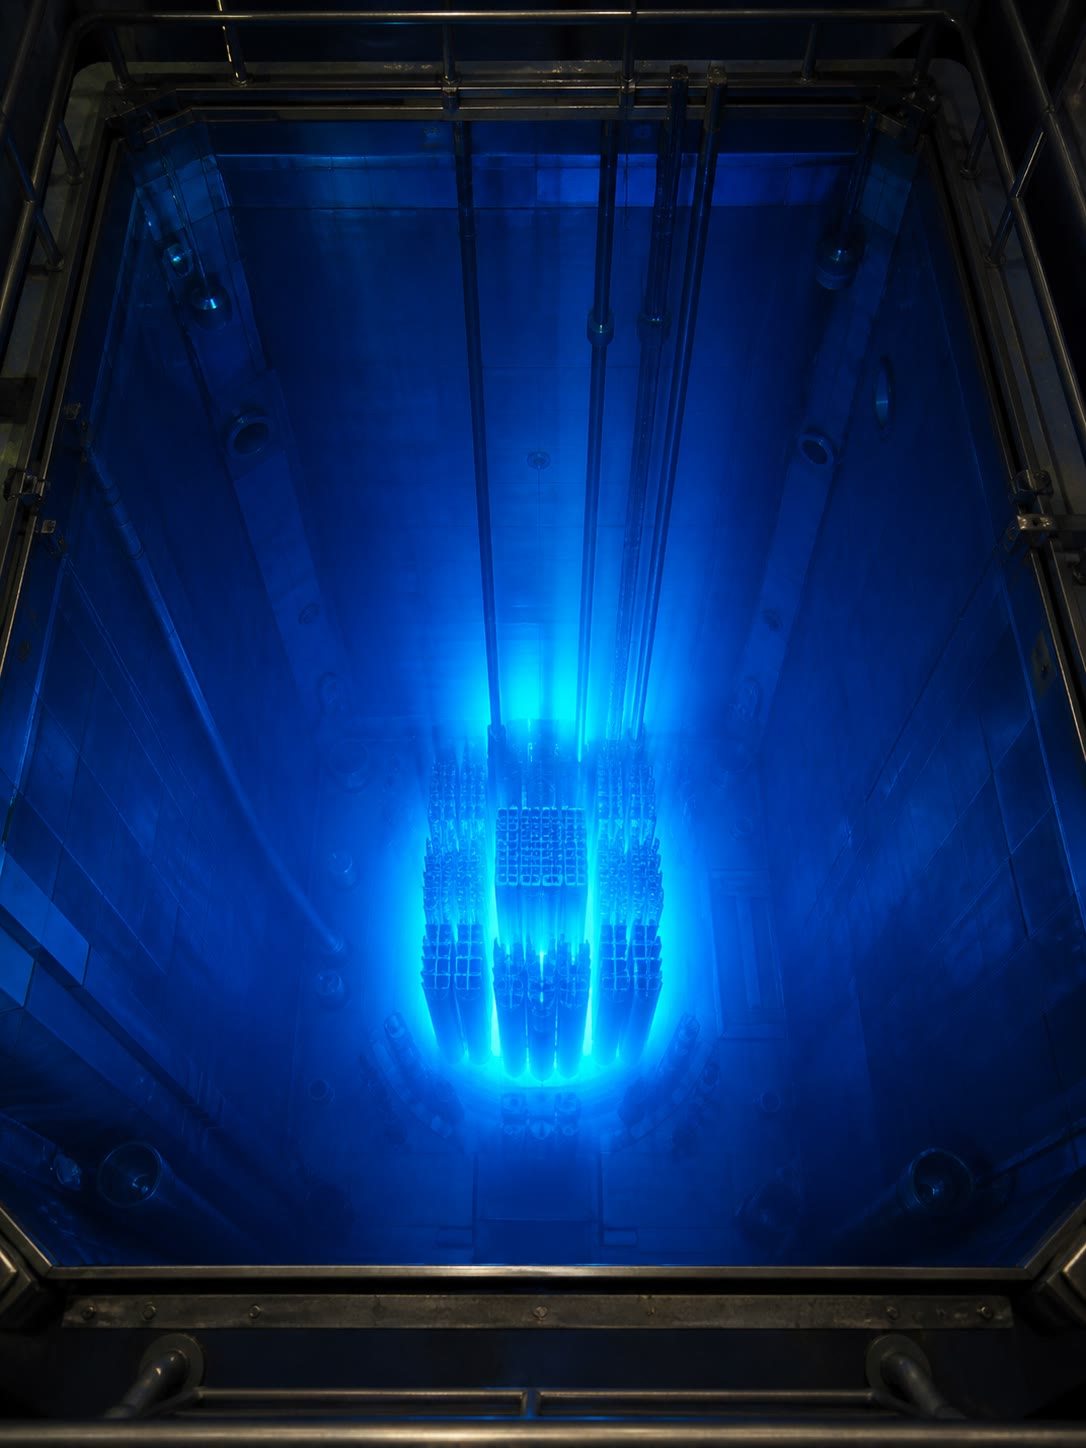
\includegraphics[width=0.45\linewidth]{images/book5/ai/b5-21-cherenkov-pool.jpg}

{\small La piscine de réacteur du problème du week-end~: les électrons $\beta$ des fragments, plus rapides que la lumière dans l'eau, enveloppent le cœur d'un bleu Tcherenkov --- le blindage, visiblement à l'œuvre.}
\end{omfigure}

\section{Problème~: journée portes ouvertes au réacteur de recherche}

\begin{problem}\label{pb:b3:nuclear-physics:1}
\emph{Journée portes ouvertes au réacteur de recherche.} Le
laboratoire national ouvre aux visiteurs son réacteur de recherche de
type piscine de \qty{20}{MW}, et vous avez obtenu une place sur la
passerelle~: en dessous, à travers huit mètres d'eau limpide, le cœur
luit d'un bleu irréel. Le guide --- un physicien des réacteurs sur le
départ --- a accepté de vous laisser faire les calculs.

\medskip\noindent\textbf{Partie I --- Le bilan d'énergie.}

\begin{enumerate}
  \item Chaque fission d'$^{235}$U libère environ \qty{200}{MeV}.
        Convertir en joules et calculer les fissions par seconde
        qui soutiennent \qty{20}{MW}.
  \item Convertir en grammes d'$^{235}$U consommés par jour.
  \item Les mêmes \qty{20}{MW} au charbon (\qty{30}{MJ/kg})~: combien
        de tonnes par jour~? Former le rapport de masses et le relier
        aux échelles en \unit{MeV} contre \unit{eV} de ce chapitre
        et de la chimie.
  \item Les fragments naissent à une liaison de
        $\sim\qty{8.5}{MeV}$ par nucléon, l'uranium à
        \qty{7.6}{MeV}~: vérifier la cohérence de
        $235\times0.9 \approx \qty{200}{MeV}$.
  \item Les fragments s'arrêtent à quelques micromètres de leur lieu
        de naissance. En quoi leurs \qty{200}{MeV} se
        convertissent-ils, et sur quelle échelle de temps cela
        atteint-il l'eau de refroidissement~?
  \item Pourquoi les fragments (par exemple $A = 95$, $Z = 36$)
        sont-ils inévitablement radioactifs~? Se servir de la
        \omterm{prop:b3:nuclear-physics:semf}{vallée de stabilité}.
\end{enumerate}

\medskip\noindent\textbf{Partie II --- Tenir $k = 1$.}

\begin{enumerate}[resume]
  \item Définir le facteur de multiplication $k$ et dites ce que
        $k = 0.999$, $1.000$, $1.001$ signifient pour la population
        de neutrons.
  \item L'eau de la piscine modère. Expliquer en deux phrases
        pourquoi ralentir les neutrons aux vitesses thermiques
        \emph{aide} à fissionner l'$^{235}$U, et pourquoi
        l'hydrogène est le meilleur modérateur (rappeler les
        chocs élastiques du volume de première année).
  \item Les barres de contrôle sont en acier au bore. Que fait le
        bore, et comment monter ou descendre les barres pilote-t-il
        $k$~?
  \item Avec les seuls neutrons prompts ($\ell = \qty{e-4}{s}$) et
        $k = 1.0005$, calculer la croissance de puissance sur une
        seconde et conclure.
  \item Les 0,7\,\% de neutrons retardés étirent le temps de
        génération effectif à $\sim\qty{0.1}{s}$~: refaites le
        calcul, et énoncer la règle de conception qui garde $k - 1$
        bien au-dessous de la fraction retardée.
  \item L'eau est aussi le caloporteur. Expliquer la sûreté
        intrinsèque~: qu'advient-il de la modération --- et donc de
        $k$ --- si l'eau s'évapore~?
  \item Pourquoi le réacteur a-t-il tout de même besoin d'un
        refroidissement de secours après l'arrêt~? (Nommer la source
        de chaleur que les barres de contrôle ne peuvent pas
        toucher.)
\end{enumerate}

\medskip\noindent\textbf{Partie III --- La lumière bleue.}

\begin{enumerate}[resume]
  \item La lueur est du rayonnement Tcherenkov~: la vitesse de la
        lumière dans l'eau vaut $c/n$ avec $n = 1.33$. Que doit faire
        une particule chargée pour en émettre~?
  \item Calculer la vitesse de seuil et, avec le
        \cref{ch:b3:relativistic-dynamics}, l'énergie cinétique de
        seuil pour un électron.
  \item Quelles particules du réacteur remplissent la condition~?
        Retracer la chaîne du fragment de fission à l'électron
        $\beta$ rapide dans l'eau.
  \item L'intensité du spectre croît vers les courtes longueurs
        d'onde~: pourquoi la piscine luit-elle en bleu plutôt qu'en
        rouge~?
  \item Le guide dit~: «~la lueur \emph{est} le blindage qui
        travaille.~» Expliquer --- que font huit mètres d'eau au
        rayonnement du cœur, et pourquoi la passerelle est-elle en
        gros sûre~?
  \item Après l'arrêt, le bleu faiblit en quelques minutes mais ne
        disparaît pas avant des jours. Relier à la question 6 de la
        partie I.
\end{enumerate}

\medskip\noindent\textbf{Partie IV --- À quoi sert le réacteur.}

\begin{enumerate}[resume]
  \item Le métier quotidien de ce réacteur est de fabriquer du
        molybdène 99 ($T_{1/2} = \qty{66}{h}$), parent du
        technétium 99m de la médecine. Pourquoi les hôpitaux du
        monde doivent-ils être réapprovisionnés chaque semaine, et
        pourquoi aucun entrepôt ne peut-il en faire des stocks~?
  \item Un envoi de \qty{100}{GBq} de Mo-99 part le lundi~;
        l'hôpital élue le Tc-99m le vendredi (96 heures plus tard).
        Quelle activité du parent reste-t-il~?
  \item Les faisceaux de neutrons issus du cœur alimentent aussi les
        instruments de diffraction du
        \cref{ch:b3:crystalline-solids}~: pourquoi les neutrons d'un
        réacteur, une fois thermalisés, naissent-ils avec la bonne
        longueur d'onde~?
  \item Le problème d'adieu du guide~: un élément combustible passe
        cinq ans en piscine avant expédition. À l'aide du mélange de
        demi-vies des fragments, expliquer la logique --- qu'ont
        acheté ces cinq ans de piscine~?
  \item Estimer la puissance résiduelle une heure après l'arrêt
        ($\approx1\,\%$ de \qty{20}{MW}) et la comparer au radiateur
        électrique d'un foyer~: un refroidissement passif par la
        piscine est-il plausible~?
  \item Refermer le bilan en quatre lignes~: $B/A$ paie
        \qty{200}{MeV} par scission~; les neutrons retardés prêtent
        les secondes qui rendent $k$ pilotable~; l'eau modère,
        refroidit, blinde et luit~; et le vrai produit du jour part
        en flacons médicaux, non en mégawatts.
\end{enumerate}
\end{problem}
